% LTeX: language=en-US

\documentclass[handout,usepdftitle=false,xcolor=dvipsnames,aspectratio=169]{beamer}
%\documentclass[beamer,usepdftitle=false,xcolor=dvipsnames,aspectratio=169]{beamer}
%\documentclass[trans,notes=show,usepdftitle=false,aspectratio=169]{beamer}
 

\usepackage[english]{babel}
\usepackage{iftex}
\ifPDFTeX
\usepackage[T1]{fontenc}
\usepackage[utf8]{inputenc}
\usepackage{lmodern}
\else
\usepackage{fontspec}
\defaultfontfeatures{Ligatures=TeX}
\setmainfont{Latin Modern Roman}
\setsansfont{Latin Modern Sans}
\setmonofont{Latin Modern Mono}
\usepackage{newunicodechar}
\newfontfamily\unicodeSymbolFont{Segoe UI Symbol}[
  BoldFont=Segoe UI Symbol,
  ItalicFont=Segoe UI Symbol,
  BoldItalicFont=Segoe UI Symbol
]
\newunicodechar{⟂}{{\unicodeSymbolFont ⟂}}
\fi
\usepackage{amsmath,amsfonts}
\usepackage{booktabs,multirow,xcolor,colortbl}
\usepackage{bm}%to use a more powerful version of \boldsymbol
\usepackage{fvextra}
\usepackage{csquotes}
\usepackage{textcomp}
\ifPDFTeX
\DeclareUnicodeCharacter{27C2}{\ensuremath{\perp}}
\fi

\newcommand{\AllSample}{ \mathcal Y^T }

\usepackage[citestyle=authoryear-comp,bibstyle=../Preamble/mystyle_lowercase,maxbibnames=5,minbibnames=1,maxnames=2, minnames=1,datezeros=false,date=long,isbn=false,url=false,backend=biber,useprefix=true]{biblatex}
\addglobalbib{../Preamble/Macro_database_biblatex.bib}	

\usepackage{upquote}
\usepackage{ragged2e}
\usepackage{microtype}

\usepackage{multimedia}
\usepackage{graphicx}
\usepackage[export]{adjustbox}
\usepackage{epstopdf}
\usepackage[labelfont=bf,format=hang, figurename=Fig.]{caption}
\usepackage[subrefformat=parens,labelformat=empty]{subcaption}
\usepackage{pgfpages} % for multiple-screen presentations

\usepackage{array}

\newcolumntype{L}[1]{>{\RaggedRight\let\newline\\\arraybackslash\hspace{0pt}}m{#1}}
\newcolumntype{C}[1]{>{\centering\let\newline\\\arraybackslash\hspace{0pt}}m{#1}}
\newcolumntype{R}[1]{>{\raggedleft\let\newline\\\arraybackslash\hspace{0pt}}m{#1}}
%https://tex.stackexchange.com/questions/12703/how-to-create-fixed-width-table-columns-with-text-raggedright-centered-raggedlef


%%% use serif font for math
\usefonttheme[onlymath]{serif}

%%% define blue highlighting
\newcommand{\highlight}[1]{{\color{blue}{#1}}}

%%%% define command for setting sources

\newcommand{\Source}{}

%%%
\beamertemplatenavigationsymbolsempty


%%% define themes
\usetheme{Boadilla}
\usecolortheme{rose}
\usecolortheme[named=blue]{structure}

\newcommand\textbox[1]{%
  \parbox{.333\textwidth}{#1}%
}

\setbeamertemplate{sections/subsections in toc}[sections numbered]


%%%% set coloring in  foot and head
\setbeamercolor{alerted text}{fg=red!80!black}
\setbeamertemplate{enumerate items}[default] % numbers enumerate items without encircling them
\setbeamertemplate{itemize items}[ball] % numbers enumerate items without encircling them
\setbeamercolor{section in head/foot}{fg=black, bg=white}
\setbeamercolor{subsection in head/foot}{fg=black, bg=white}
\setbeamercolor{title}{fg=black}
\setbeamercolor{subtitle}{fg=blue}

\setbeamertemplate{caption}[numbered]

%%% set overlays as default
\beamerdefaultoverlayspecification{<+->}

%%%% settings for output mode

\mode<beamer>
{
%\setbeameroption{show notes on second screen=right}
}

\mode<trans>
{\renewcommand{\highlight}[1]{{\textbf{#1}}}}


\mode<handout>
{
\renewcommand{\highlight}[1]{{\textbf{#1}}}
%\pgfpagesuselayout{4 on 1}[a4paper,border shrink = 5mm,landscape]
%\setbeamercolor{background canvas}{bg=black!5}
}


%%% define Exercise counter
\newcounter{Exercise}
\resetcounteronoverlays{Exercise}
\setcounter{Exercise}{0}
\newcommand{\Exercise}{\refstepcounter{Exercise}\emph{\structure{Übung \theExercise}: }}

%%%% define environments for theorems etc and make them numbered
\setbeamertemplate{theorems}[numbered]

\newtheorem{assum}{Assumption}
\setbeamertemplate{assum}[numbered]

\newtheorem{defin}{Definition}
\setbeamertemplate{defin}[numbered]

\newtheorem{propos}{Proposition}
\setbeamertemplate{propos}[numbered]


%%%% Make Parts show up in TOC
\makeatletter
\AtBeginPart{%
  \addtocontents{toc}{\protect\beamer@partintoc{\the\c@part}{\beamer@partnameshort}{\the\c@page}}%
}
%% number, shortname, page.
\providecommand\beamer@partintoc[3]{%
  \ifnum\c@tocdepth=-1\relax
    % requesting onlyparts.
    \makebox[6em]{#1.} #2
    \par
  \fi
}
\define@key{beamertoc}{onlyparts}[]{%
  \c@tocdepth=-1\relax
}
\makeatother%

%%%% fix bug in beamer package with note itemize
%%% http://tex.stackexchange.com/questions/1480/changing-the-textwidth-of-the-notes-in-beamer-repost-from-so
\makeatletter
\defbeamertemplate{note page}{infolines}
{%
  \vskip.75em
  \nointerlineskip
  \begin{minipage}{\textwidth} % this is an addition
  \footnotesize \insertnote
  \end{minipage}               % this is an addition
}
\makeatother

\setbeamertemplate{note page}[infolines]


\newcommand{\backupbegin}{
   \newcounter{framenumberappendix}
   \setcounter{framenumberappendix}{\value{framenumber}}
}
\newcommand{\backupend}{
   \addtocounter{framenumberappendix}{-\value{framenumber}}
   \addtocounter{framenumber}{\value{framenumberappendix}}
}

\hypersetup{bookmarksnumbered=true,naturalnames=true,pdfhighlight=/N,citebordercolor={1 1
1},linkbordercolor={1 1 1},colorlinks=true,anchorcolor=black,linkcolor=blue,citecolor=green,urlcolor=green,
pdfpagemode=UseOutlines,breaklinks=true,
pdfkeywords=Dynare, pdfsubject=Dynare,pdfstartpage=1} %pdfpagemode=fullpage

\usepackage[copyright]{ccicons}

\usepackage{tikz,pgfplots}
\pgfplotsset{compat=1.18}
\usetikzlibrary{arrows,calc,decorations.pathreplacing,decorations.shapes}
\pgfdeclarelayer{background}
\pgfdeclarelayer{foreground}
\pgfsetlayers{background,main,foreground}

\usepackage{relsize}
\newcommand\LM{\ensuremath{\mathit{LM}}}
\newcommand\IS{\ensuremath{\mathit{IS}}}
\DeclareMathOperator{\std}{std}


\setbeamertemplate{footline}{
\begin{beamercolorbox}{subsection in head/foot}
\insertsectionnavigationhorizontal{.95\textwidth}{\hskip0pt
\hfill}{\hfill \insertframenumber /\inserttotalframenumber}
\end{beamercolorbox}
}

\newenvironment{witemize}{\itemize\addtolength{\itemsep}{8pt}}{\enditemize}
\newenvironment{wenumerate}{\enumerate\addtolength{\itemsep}{8pt}}{\endenumerate}

\usepackage[]{minted}
\usepackage{tcolorbox}
\usepackage{etoolbox}
\BeforeBeginEnvironment{minted}{\begin{tcolorbox}[boxsep=0mm]}%
\AfterEndEnvironment{minted}{\end{tcolorbox}}%

\AtBeginEnvironment{minted}{%
  \renewcommand{\fcolorbox}[4][]{#4}}  


\begin{document}

%\inserttotalframenumber


\title[]{\textbf{Advanced Dynare\\}
  \medskip{Chapter V}\\
  \emph{Kalman Filter and the likelihood}
}

\author{Johannes Pfeifer}
\input{../date_place.txt}

\AtBeginSection[]
{
  \begin{frame}
    \frametitle{Outline}
    \tableofcontents[currentsection]
  \end{frame}
}

\maketitle

\begin{frame}
  \frametitle{Outline}
  \tableofcontents%[onlyparts]
\end{frame}




%\begin{frame}
%\frametitle{Outline}
%\tableofcontents[sectionstyle=show]
%\end{frame}
\begin{frame}{Cool stuff}

  \begin{center}
    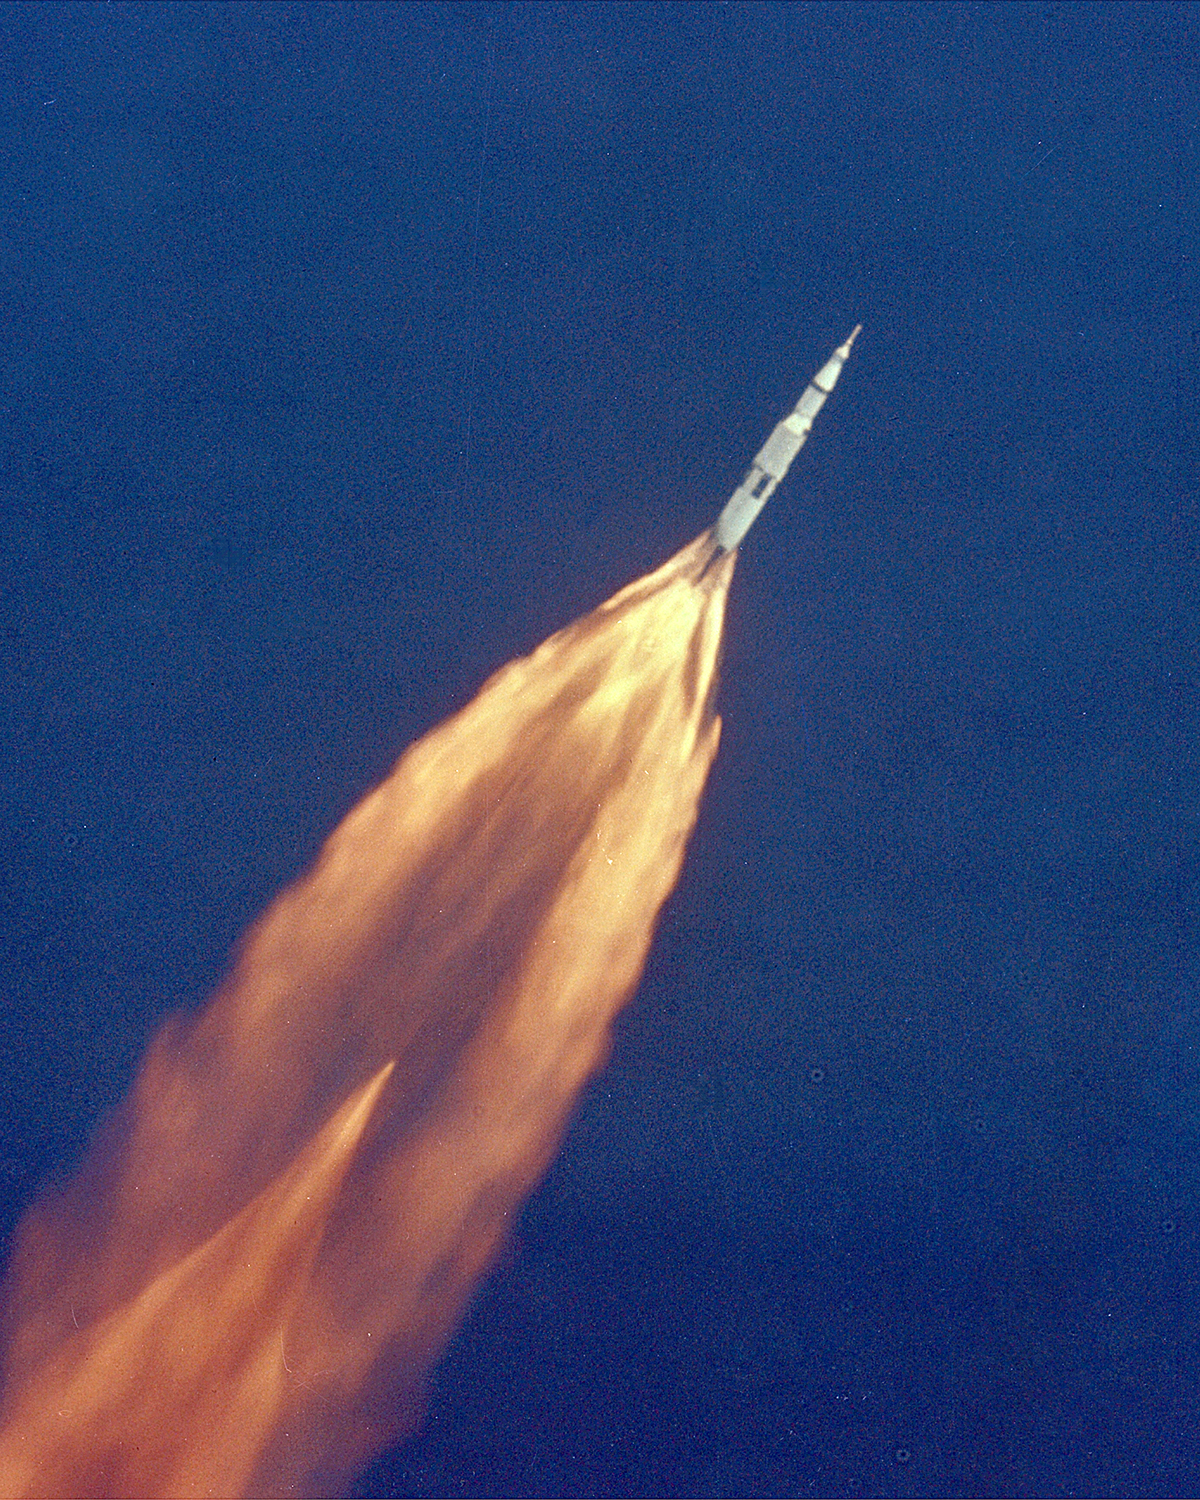
\includegraphics[scale=0.6]{Figures/apollo11}
  \end{center}

\end{frame}
\note{ Kalman filtering rapidly became a mainstay of aerospace engineering. It was used, for example, in the Ranger, Mariner, and Apollo missions of the 1960s.

  In particular, the on-board computer that guided the descent of the Apollo 11 lunar module to the moon had a Kalman filter. }

\begin{frame}{The basic concept}
  \begin{itemize}
    \item named after seminal work of \textcite{Kalman1960} and \textcite{KalmanBucy1961}
  \end{itemize}
  %
  \begin{figure}
    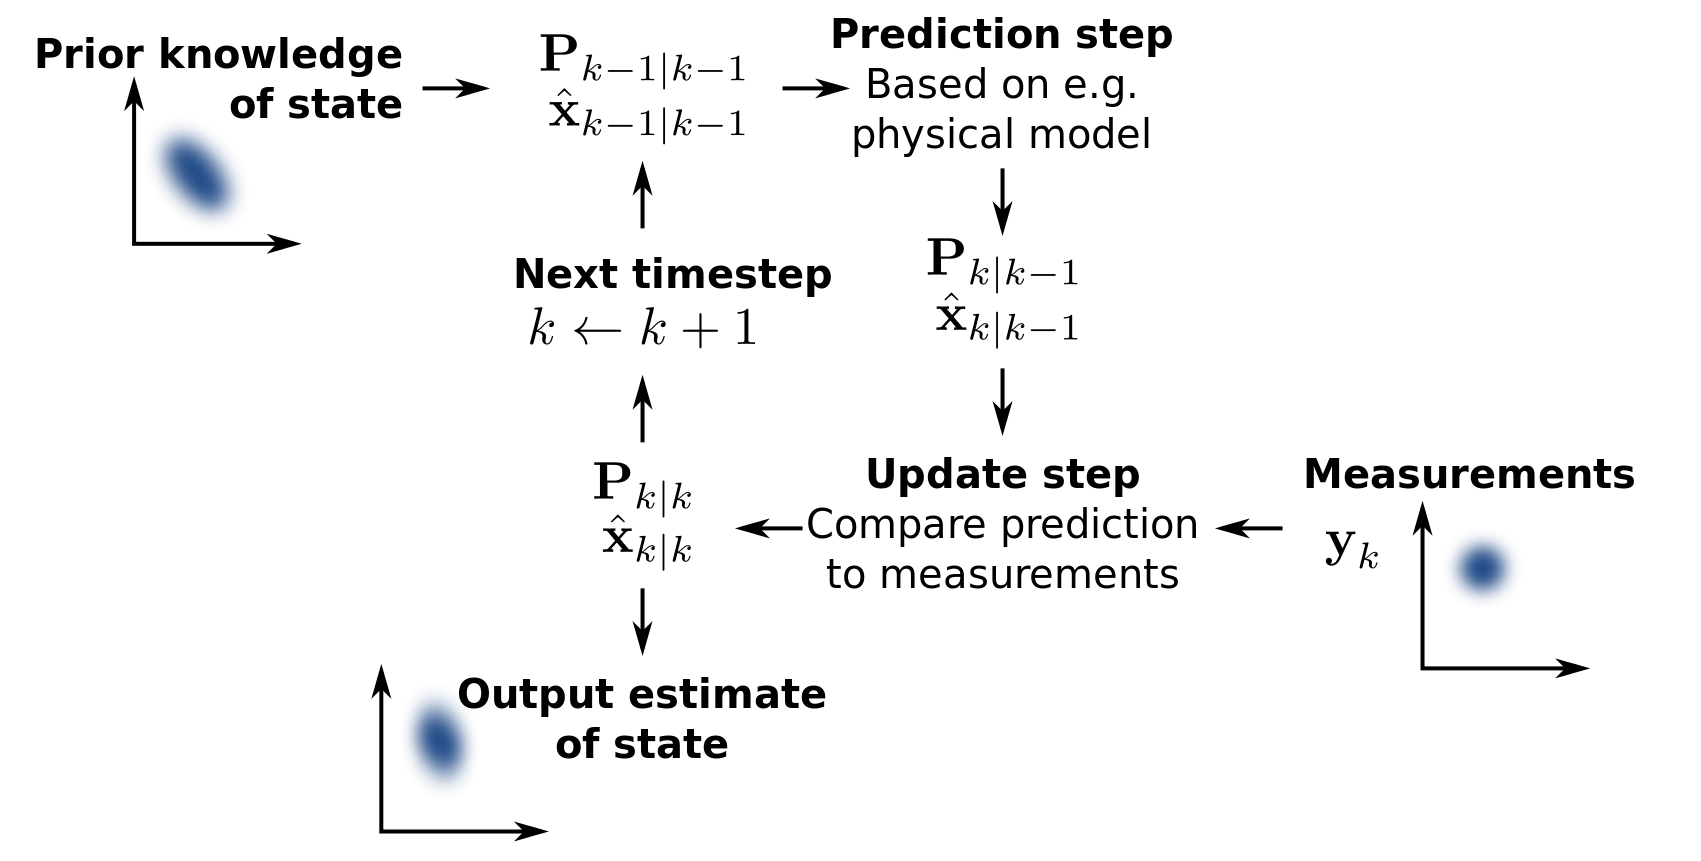
\includegraphics[scale=0.2]{Figures/Basic_concept_of_Kalman_filtering}
    \caption{Source: ``Basic concept of Kalman filtering'' by Petteri Aimonen}

  \end{figure}
  %
\end{frame}


\begin{frame}{References}
  \begin{itemize}
    \item Handout online\vspace{0.2cm}
    \item \textcite[][Chapter 2.5]{LjungqvistSargent2012}\vspace{0.2cm}
    \item \textcite[][Chapter 13]{Hamilton1994}\vspace{0.2cm}
    \item \textcite{DurbinKoopman2012}\vspace{0.2cm}
    \item \textcite[][Chapter 6]{Canova2007Book}
  \end{itemize}

\end{frame}


\section{Setup}
\begin{frame}{Gaussian state space}
  \begin{itemize}
    \item Solution to linearized RBC model took \highlight{state space form}, which can be written as
  \end{itemize}
  \begin{align}
    x_{t + 1} & = F x_t + w_{t + 1},\; w_{t + 1}\mathop  \sim \limits^{iid} \mathcal{N}\left(0,Q\right) \\
    y_t       & = Hx_t + \nu_t, \; \nu _t\mathop  \sim \limits^{iid} \mathcal{N}\left(0,R \right)
  \end{align}

  \begin{itemize}
    \item $F,H,Q,R$ are functions of the model parameters $\theta$
    \item $x_t$ is an $n_x \times 1$ vector of states\vspace{0.2cm}
    \item $y_t$ is an $n_y \times 1$ vector of observables\vspace{0.2cm}
    \item $w_t$ is a $p \times 1$ vector of structural errors\vspace{0.2cm}
    \item $\nu_t$ a vector of measurement errors\vspace{0.2cm}
    \item Assumption: $w_t$ and $\nu_t$ are orthogonal
          \begin{equation*}
            \mathbb{E}_t\left( w_{t + 1}\nu_s \right) = 0 \quad \forall\; t+1 \text{ and } s\geq0
          \end{equation*}
  \end{itemize}
\end{frame}

\begin{frame}{Fundamental problem: unobserved states}

  \begin{itemize}
    \item This implies that
          \begin{equation}
            y_t = H\left( {F{x_{t - 1}} + {w_t}} \right) + {\nu _t}
          \end{equation}
    \item Thus, $y_t$ is normally distributed:
          \begin{equation}
            y_t\sim \mathcal{N}(HFx_{t-1},HQH' + R) \label{eq:distribution_y}
          \end{equation}
    \item If all states were observed, we could directly construct the likelihood $f(y_T,\dots,y_1|\theta)$\vspace{0.2cm}
    \item We could then run optimizer over our estimated parameter set $\tilde \theta \subseteq \theta $ to get ML estimate of $\tilde \theta$\vspace{0.2cm}
    \item Problem: we have \highlight{unobserved states} and cannot use equation \eqref{eq:distribution_y}\vspace{0.2cm}
    \item Solution: turn to Kalman filter to back out states from the observed data\\
          $\rightarrow$ \highlight{Filtering problem}
  \end{itemize}
\end{frame}



\begin{frame}{Initial values for states}

  \begin{witemize}
    \item Initial value $x_0$ distributed as
    \begin{equation}
      x_0 \sim \mathcal{N}\left(\hat{x}_{0|-1},\Sigma_{0|-1} \right)
    \end{equation}
    \item subscript $-1$ denotes information at the beginning of times\vspace{0.2cm}
    \item particular observation: $y_t$ \vspace{0.2cm}
    \item complete history of observations up to a certain point in time: $y^t=\{y_t,\ldots,y_0\}$\vspace{0.2cm}
    \item What does this imply for $y_0= H{x_0} + {\nu _0}$?
  \end{witemize}
\end{frame}

\begin{frame}{Initial values for observables}

  \begin{itemize}
    \item Let's define
          \begin{equation}
            \hat y_{0|-1} \equiv E({y_0}|y^{-1}) =E( H{x_0} + {\nu _0}|y^{-1})=H\hat x_{0|-1}
          \end{equation}
    \item \highlight{Mean Squared Error} of ${y_0}$ given information up to $t=-1$
          \begin{align}
             & E\left[\left( y_0 - \hat y_{0|-1} \right)\left( y_0 - \hat y_{0|-1} \right)'|y^{-1}\right]\notag   \\& = E\left[\left( {H{x_0} + {\nu _0}-H\hat x_{0|-1}} \right)\left( {H{x_0} + {\nu _0}-H\hat x_{0|-1}} \right)'|y^{-1}\right] \notag\\
             & =  E\left[ {H{(x_0-\hat x_{0|-1})}{(x_0-\hat x_{0|-1})}'H' + {\nu_0}{\nu_0}'}|y^{-1}\right] \notag \\
             & = H{\Sigma _{0|-1}}H' + R
          \end{align}
    \item  Hence:
          \begin{equation}
            {y_0} \sim N\left( {H{{\hat x}_{0|-1}},H{\Sigma _{0|-1}}H' + R} \right)
          \end{equation}

  \end{itemize}
\end{frame}

\begin{frame}{What's the goal?}

  \begin{itemize}
    \item Economist only observes the observables: $y^t=\{y_t,\ldots,y_0\}$\vspace{0.2cm}
    \item Wants to infer the \highlight{unobserved state variables} $x_t,\ldots,x_0$\vspace{0.2cm}
    \item Assumption: Economist knows state space structure, i.e.\ $H,F,R,Q$\vspace{0.2cm}
    \item Aim: find \highlight{recursive} formulas for the state forecast
          \begin{equation}
            \hat x_{t|t-1}\equiv E[x_t|y^{t-1}]
          \end{equation}
          and the Mean Squared Error/covariance matrices of the forecast error (FE)
          \begin{equation}
            \Sigma _{t|t-1} \equiv E\left[ \left( x_t - {\hat x}_{t|t-1} \right)\left( x_t - {\hat x}_{t|t-1} \right)'|y^{t - 1} \right]
          \end{equation}
    \item Recursiveness allows for online tracking

  \end{itemize}
\end{frame}

\begin{frame}{Idea}
  \begin{itemize}
    \item regression of the (unknown) state FE on observation FE
          \begin{equation}
            {x_t} - {{\hat x}_{t|t-1}} = L_t\left( {{y_t} - \hat y_{t|t-1}} \right) + \eta_t
          \end{equation}
          $L_t$: regression coefficient; $\eta_t$: regression residual\vspace{0.2cm}

    \item Forecast $\hat y_{t|t-1}$ of $y_t$ given by
          \begin{equation}
            \hat y_{t|t-1}=H\hat x_{t|t-1}
          \end{equation}

    \item regression equation can then be written as
          \begin{equation}\label{eq:regression}
            {x_t} - {{\hat x}_{t|t-1}} = L_t\left( {{y_t} - H{{\hat x}_{t|t-1}}} \right) + \eta_t
          \end{equation}

    \item Problem: don't know the left-hand side $\Rightarrow$ can't compute $L_t$\vspace{0.2cm}
    \item But: if we somehow knew $L_t$, could form a forecast of our state FE
  \end{itemize}
\end{frame}

\section[Recursion]{Filter recursion}
\begin{frame}{Computing $L_t$}
  \begin{itemize}
    \item Goal: compute $L_t$ at time $t$\vspace{0.2cm}
    \item General formula for a \highlight{population regression}
          \begin{equation*}
            \beta  = E\left(YX'\right)\left[ E\left( XX' \right) \right]^{-1}
          \end{equation*}
    \item In our case
          \begin{align}
            L_t = & E\left[\left( {{x_t} - {\hat x}_{t|t-1}} \right)\left( y_t - H\hat{x}_{t|t-1} \right)' \right]\notag                            \\
                  & \times{\left(E\left[ \left( y_t - H\hat{x}_{t|t-1} \right)\left( y_t - H\hat{x}_{t|t-1} \right)' \right] \right)^{ - 1}} \notag \\
            =     & \; \Sigma _{t|t-1}H'\left(H\Sigma_{t|t-1}H' + R \right)^{ - 1}
          \end{align}
  \end{itemize}
\end{frame}

\begin{frame}{Stochastic singularity}
  \begin{witemize}
    \item Computation requires $\left(H\Sigma_{t|t-1}H' + R \right)^{ - 1}$
    \item For the inversion, state-space model must not feature \highlight{stochastic singularity}, i.e. the forecast error matrix of the observables must have full rank
    \item Typical requirement: at least as many shocks as observables
    \item Having more shocks than observables is not a problem
    \item Also requires that there is no collinearity between observables
    \item[$\rightarrow$] Problem if, e.g., all components of budget constraint are observed
    \item Way out: add measurement error \parencite[see][]{Altug1989,Sargent1989,Ireland2004}
    \item May also help with model mis-specification \parencite{DelNegroSchorfheide2009}
  \end{witemize}
\end{frame}


\begin{frame}{Updating step: forecasting $x_1$}
  \begin{itemize}
    \item Rewrite state transition equation
          \begin{align}
            {x_{1}} & = F{x_0} + {w_{1}}\notag                                                                                                                    \\
                    & =F{{\hat x}_{0|-1}} + F\left( {{x_0} - {{\hat x}_{0|-1}}} \right) + {w_{1}} \notag                                                          \\
                    & \overset{\eqref{eq:regression}}{=} F{{\hat x}_{0|-1}} + F\left( {L_0\left( {{y_0} - H{{\hat x}_{0|-1}}} \right) + \eta_0} \right) + {w_{1}}
          \end{align}
    \item Forecast tomorrow's state just based on yesterday's forecast and today's observation
          \begin{align}
            \hat x_{1|0}=E\left[ {{x_{1}}|{y^0}} \right] & = F{{\hat x}_{0|-1}} + \underbrace {FL_0}_{K_0}\left( {{y_0} - H{{\hat x}_{0|-1}}} \right)\notag %\\&=F{{\hat x}_{0|-1}} + {K_0}\left( {{y_0} - H{{\hat x}_{0|-1}}} \right)
          \end{align}
    \item \highlight{Kalman Gain}
          \begin{equation}
            K_0=FL_0=F{\Sigma _{0|-1}}H'{\left( {H{\Sigma _{0|-1}}H' + R} \right)^{ - 1}} \label{eq:KalmanGain}
          \end{equation}
          $\rightarrow$ how much is state estimate updated based on previous FE
  \end{itemize}
\end{frame}

\begin{frame}{$x_2$, $x_3$,\ldots ?}
  \begin{itemize}
    \item We want to use population regression
          \begin{equation*}
            L_1 = \Sigma _{1|0}H'\left(H\Sigma_{1|0}H' + R \right)^{ - 1}
          \end{equation*}
    \item For this, we need covariance/mean squared error matrix $\Sigma_{1|0}$
          \begin{align}
            \Sigma_{1|0}= & E\left[\left( {{x_1} - {{\hat x}_{1|0}}} \right)\left( {{x_1} - {{\hat x}_{1|0}}} \right)'|y^0\right]\notag \\
            =             & \left( {F - {K_0}H} \right){\Sigma _{0|-1}}\left( {F - {K_0}H} \right)' + Q + {K_0}R{K_0}'
          \end{align}

    \item From this, we now know that
          \begin{equation}{x_1} \sim \mathcal{N}\left( {{{\hat x}_{1|0}},{\Sigma _{1|0}}} \right)\end{equation}
    \item We can now start over again, delivering the recursion we were looking for
  \end{itemize}
\end{frame}

\begin{frame}{Summary}
  At time t, given $\hat x_{t|t-1},\Sigma_{t|t-1}$ and observing $y_t$\vspace{0.2cm}
  \begin{enumerate}
    \item Compute the forecast error in the observations using
          \begin{equation}
            a_t= y_t-H\hat x_{t|t-1}
          \end{equation}
    \item Compute the \highlight{Kalman Gain} $K_t$ using
          \begin{equation}\label{eq:filtering_step}
            K_t=F{\Sigma _{t|t-1}}H'{\left( {H{\Sigma _{t|t-1}}H' + R} \right)^{ - 1}}
          \end{equation}
    \item Compute the state forecast for next period given today's information
          \begin{equation}
            \hat x_{t+1|t}=F{{\hat x}_{t|t-1}} + K_t\left( {{y_t} - H{{\hat x}_{t|t-1}}} \right)=F{{\hat x}_{t|t-1}} + K_ta_t
          \end{equation}
    \item Update the covariance matrix
          \begin{equation}
            \Sigma_{t+1|t} = \left( {F - {K_t}H} \right){\Sigma _{t|t-1}}\left( {F - {K_t}H} \right)' + Q + {K_t}R{K_t}' \label{eq:Sigma_tp1givent}
          \end{equation}
  \end{enumerate}
\end{frame}


\section[Initialization]{Filter initialization}
\begin{frame}{Initialization}
  \begin{itemize}
    \item How to initialize filter at $t=0$ where no observations are available?\\\vspace{0.2cm}
          $\rightarrow$ start with \highlight{unconditional} mean $E(x)$ and Variance $\Sigma$\vspace{0.2cm}
    \item Given covariance stationarity, the unconditional mean is
          \[
            E(x)=E{x_{t + 1}} = E(F{x_t} + {w_{t + 1}})=FE(x) \Rightarrow (I-F)E(x)=0
          \]
          hence, $E(x)=0$\vspace{0.2cm}
    \item For the covariance matrix, we have
          \begin{align}
            \Sigma & =E\left[\left( {F{x_t}+ {w _t}} \right)\left( {F{x_t} + {w _t}} \right)'\right]\notag \\
                   & = {E}\left[ {F{x_t}{x_t}'F' + {w_t}{w_t}'} \right]\notag                              \\
                   & = F\Sigma F' + Q
          \end{align}
          $\rightarrow$ so-called \highlight{Lyapunov-equation}
  \end{itemize}
\end{frame}

\begin{frame}{Initialization: the slow solution}
  \begin{itemize}
    \item If $A,B,C$ are conformable matrices
          \[
            vec(ABC)=(C'\otimes A)vec(B)
          \]
    \item Hence
          \[
            vec(\Sigma)=(F\otimes F)vec(\Sigma)+vec(Q)
          \]
    \item This has solution
          \begin{equation}
            vec(\Sigma)=\left(I_{n_x^2}-(F\otimes F)\right)^{-1}vec(Q)
          \end{equation}
    \item Problem: Inversion of $n_x^2$ matrix $\rightarrow$ sloooooow\vspace{0.2cm}
  \end{itemize}
\end{frame}

\begin{frame}[fragile]{Lyapunov solvers in Dynare}
  \begin{witemize}
    \item Dynare offers a menu of superior alternatives via the
    \begin{minted}{c++}
lyapunov = OPTION
  \end{minted}
    \item The \texttt{lyapunov=default} option uses the Schur decomposition-based Bartels-Stewart algorithm
    \item  The \texttt{lyapunov=doubling} option uses the doubling algorithm, which is usually a lot faster for large models
    \item For big models, the \texttt{lyapunov=square\_root\_solver} of MATLAB's Control System Toolbox may also work well
  \end{witemize}
\end{frame}

\begin{frame}{Initialization: Diffuse Kalman filter}
  \begin{itemize}
    \item Consider model with unit root: does not violate \textcite{BlanchardKahn1980} conditions\vspace{0.2cm}
    \item Problem: unconditional variance does not exist for some variables, only the conditional one\vspace{0.2cm}
    \item[$\rightarrow$] cannot use unconditional one for initialization\vspace{0.2cm}
    \item Alternative: \highlight{diffuse Kalman filter} \parencite{Dejong1991,KoopmanDurbin2003} that considers initial state as diffuse vector (let variance go to infinity)\vspace{0.2cm}\\
          $\rightarrow$ requires specifying the \texttt{diffuse\_filter}-option of Dynare (also important for treating unit roots as being stable (\texttt{options\_.qz\_criterium}))

  \end{itemize}
\end{frame}


\begin{frame}
  \frametitle{Diffuse initialization of the filter}

  \begin{witemize}
    \item Vector $ x $ is split in $ \begin{bmatrix} x^1 & x^2 \end{bmatrix} $, where $ x^1 $ contains non-stationary variables and $x^2$ stationary ones
    \item \textcite{KoopmanDurbin2003} compute second order expansion of the Kalman filter formulas when the variance of the non-stationary variables tends toward infinity
    \item Initial values for the state variables are $ x^1_{0|-1} =x^2_{0|-1}= 0 $\\
    $\rightarrow$ unconditional mean of the stationary elements in $ x_t $, with no effect for non-stationary ones
  \end{witemize}

\end{frame}

\begin{frame}{Diffuse filter: initial co-variance matrix}
  \begin{witemize}
    \item The initial co-variance matrix is
    \begin{equation}
      P_{0|-1} = P^{\infty}_{0|-1} + P^{*}_{0|-1} = \begin{bmatrix} I & 0 \\ 0 & 0 \end{bmatrix} + \begin{bmatrix} 0 & 0 \\ 0 & \Sigma_{x_2} \end{bmatrix} \: ,
    \end{equation}
    where
    \begin{itemize}
      \item the identity matrix $I$ of the same dimensions as $ F_{11}$ is the diffuse prior on the initial values of the stochastic trends
      \item $ \Sigma_{x_2} $ is the co-variance matrix of the stationary part of $x_t$, i.e.\ $x_t^2$
    \end{itemize}
    \item Schur decomposition can be used to find the actual number of unit roots\\
    $\rightarrow$ important if model has co-integrated variables
    \item While $P^{\infty}_{t|t-1}$ is different from zero, the filter is in a diffuse step
  \end{witemize}

\end{frame}

\begin{frame}{Exiting the diffuse filter}
  \begin{witemize}
    \item For non-degenerate models that are informative about the state of the world, the number of diffuse steps $d$ is smaller than $t$\\
    $\rightarrow$ algorithm falls back on standard recursions where $x_{d|d-1},P_{d|d-1}$ can be used for initialization
    \item However, diffuse filter would never exit with only stationary observables\\
    $\rightarrow$ if non-stationary states are not projected onto some observation, they provide no information about state location
    \item Dynare automatically tests if there exist unit roots not projected onto any observable\\
    $\rightarrow$ set entries of $P_{0|-1}^{\infty}$ associated to such state automatically to 0
    \item If only unobserved non-stationary states:  $P_{0|-1}^{\infty}$  has rank zero\\
    $\rightarrow$ use standard Kalman filter using $P_{0|-1}^*$
    \item Typical example: inflation rates are not informative about price level in model
  \end{witemize}

\end{frame}

\begin{frame}
  \frametitle{Problem with co-integrated variables and improper prior}
  \begin{witemize}
    \item The diffuse prior is improper: no direct comparison of marginal data density of different models is possible\\
    $\rightarrow$ Special care (i.e.\ presample) must be used for models comparison
    \item Dynare internally works with non-stationary trends instead of non-stationary variables
    \item Core problem otherwise: when $x^1_t$ contains co-integrated variables, the limit co-variance matrix of the diffuse state vector is not given by $\lim_{k \to \infty} kI$\\
    $\rightarrow$ diffuse prior on all involved states would imply too much volatility of initial conditions (efficiency of filter/smoother drastically deteriorates)
    \item Dynare therefore employs a Schur decomposition to isolate trends corresponding to different unit roots\\
    $\rightarrow$ work directly with stochastic trends instead of trending variables by rotating the variable space
    \item Requires resorting to univariate diffuse Kalman filter recursions \parencite{KoopmanDurbin2000}
  \end{witemize}
\end{frame}

\begin{frame}{Univariate Kalman filter}

  \begin{witemize}
    \item The updating step using the Kalman gain involves inversion of potentially big matrix
    \begin{equation}\tag{\ref{eq:filtering_step}}
      K_t=F{\Sigma _{t|t-1}}H'{\left( {H{\Sigma _{t|t-1}}H' + R} \right)^{ - 1}}
    \end{equation}
    \item \textcite{KoopmanDurbin2000}: update state prediction sequentially using one observed series at a time instead of using the full vector of observations\\
    $\rightarrow$  avoids matrix inversion
    \item Univariate Kalman filter
    \begin{itemize}
      \item can provide decent speed-up for large models
      \item works even if there is stochastic singularity
    \end{itemize}
    \item However: stochastic singularity typically indicates a problem with the model that cannot simply be solved with a different filter!
  \end{witemize}

\end{frame}


\begin{frame}{Fast Kalman filter}

  \begin{witemize}
    \item Most expensive computation involves updating the covariance matrix
    \begin{equation}
      \Sigma_{t+1|t} = \left( {F - {K_t}H} \right){\Sigma _{t|t-1}}\left( {F - {K_t}H} \right)' + Q + {K_t}R{K_t}' \tag{\ref{eq:Sigma_tp1givent}}
    \end{equation}
    due to first part involving multiplication of three $n_x \times n_x$ matrices: $\mathcal{O}(n_x^3)$
    \item Central insight: $\Sigma_{t+1|t}$ is rarely full rank
    \item Idea: use a rank reduction technique that considers differences in state variances
    \begin{equation}
      \Delta \Sigma_{t|t-1}=W_tM_tW_t' \: ,
    \end{equation}
    where $rank(M_t)$ is at most $min(n_x,n_y)$\\
    $\rightarrow$ allows large speed-up if model has many more states than observables (\textcite{SmetsWouters2007} has 50 states but only 7 observables)
  \end{witemize}

\end{frame}


\begin{frame}
  \frametitle{Chandrasekhar recursion}
  \begin{itemize}
    \item \textcite{Herbst2015} suggests the following implementation of Chandrasekhar recursion
          \begin{align}
            G_t & = G_{t-1} + HW_{t-1}M_{t-1}W'_{t-1}H'                    \\
            K_t & = K_{t-1} + FW_{t-1}M_{t-1}W'_{t-1}H'                    \\
            W_t & = (F - K_tG_tH)W_{t-1}                                   \\
            M_t & = M_{t-1} + M_{t-1}W'_{t-1}H'G^{-1}_{t-1}HW_{t-1}M_{t-1}
          \end{align}
          with initialization
          \begin{align}
            G_1 & = H\Sigma_0H' + RQR \\
            K_1 & = F\Sigma_0H'       \\
            W_1 & = K_1               \\
            M_1 & = -G^{-1}_1
          \end{align}
    \item Recursion only works if $\Sigma_0$ exists\\
          $\rightarrow$ not suitable for models with unit roots
  \end{itemize}
\end{frame}

\begin{frame}{Steady State Kalman filter}
  \begin{itemize}
    \item It can be shown that the matrix recursions in the Kalman filter converge \parencite[See][Chapter 13.5]{Hamilton1994}\vspace{0.2cm}
    \item Kalman gain and forecast error variance matrix will settle on final values \vspace{0.2cm}
    \item Continuing with recursions after they have settled within reasonable tolerance is computationally expensive\vspace{0.2cm}
    \item[$\rightarrow$] check for convergence and then continue with fixed matrices\vspace{0.2cm}
    \item Dynare by default uses this \highlight{steady state Kalman filter}
  \end{itemize}
\end{frame}

\begin{frame}[fragile]{Heteroskedastic filter}
  \begin{itemize}
    \item Our description used time-invariant matrices state space matrices $H,F,Q,R$, but Kalman filter can accommodate time-varying ones
    \item Somewhat problematic from the perspective of rational expectations modeling as implied structural breaks are essentially MIT shocks
    \item Dynare has \texttt{heteroskedastic\_filter} option to allow heteroskedasticity via $Q_t$
          \small
          \begin{minted}{c++}
heteroskedastic_shocks;
var e1;
periods 86:87, 89:97;
scales 0.5, 0;
var e1;
periods 88;
values 0.1;
  \end{minted}
    \item Can e.g.\ by used for increasing variance in Covid period
  \end{itemize}
\end{frame}


\begin{frame}{Options in Dynare}
  \begin{witemize}
    \item \texttt{kalman\_algo = INTEGER}
    \begin{itemize}
      \item[0] automatically use Multivariate Kalman Filter for stationary models and Multivariate Diffuse Kalman Filter for non-stationary models
      \item[1] Use Multivariate Kalman Filter
      \item[2] Use Univariate Kalman Filter
      \item[3] Use Multivariate Diffuse Kalman Filter
      \item[4] Use Univariate Diffuse Kalman Filter
    \end{itemize}
    \item \texttt{lik\_init = INTEGER}
    \begin{itemize}
      \item[1] Use unconditional variance
      \item[3] Use diffuse initialization\\
            $\rightarrow$ better to use \texttt{diffuse\_filter}-option
    \end{itemize}
    \item \texttt{fast\_kalman\_filter}: use Chandrasekhar recursions

  \end{witemize}
\end{frame}

\begin{frame}{Kalman smoothing and other outputs}
  \begin{itemize}
    \item The Kalman filter recursions provide us with \highlight{filtered variables} $\mathbb{E}_t{x_{t+1}}$, i.e.\ the best prediction for tomorrow's state given information up to today\vspace{0.2cm}
    \item We can also compute \highlight{updated variables} $\mathbb{E}_t{x_{t}}$, i.e.\ our best estimate of the state today given information up to today (remember that $x_t$ is not in the information set here!)\vspace{0.2cm}
    \item Note: the terminology here follows Dynare as there seems to be no standard for naming these two objects\vspace{0.2cm}
    \item More importantly, we are regularly interested in our best estimates of shocks and states given the full observed data up to time $T$\vspace{0.2cm}
    \item The \highlight{Kalman Smoother} provides recursions for obtaining these estimates \highlight{$\mathbb{E}_T(x_t)$} and \highlight{$\mathbb{E}_T(w_t)$} by working backwards in time (for details, see the handout)
  \end{itemize}
\end{frame}


\section[Likelihood]{Constructing the likelihood}
\begin{frame}{From filtering to estimation}
  \begin{itemize}
    \item Typically we are not interested in filtering per se, but rather in estimating a model
    \item Start with complete history of observables up to time $t$: $y^t=\{y_t,\ldots,y_0\}$\vspace{0.2cm}
    \item Likelihood function $f\left( {{y_T},\ldots,{y_0}} \right)$ can be factored as
          \[
            f\left( {{y_T},\ldots,{y_0}} \right) = f\left( {{y_T}|{y^{T - 1}}} \right)\times f\left( {{y_{T - 1}}|{y^{T - 2}}} \right)\times \ldots \times f\left( {{y_1}|{y^0}} \right)\times f\left( {{y_0}} \right)
          \]
    \item Earlier we derived
          \[
            y_t \sim \mathcal{N}\left( H\hat x_{t|t-1},\underbrace{H{\Sigma _{t|t-1}}H' + R}_{\equiv \Omega_t} \right)
          \]

  \end{itemize}
\end{frame}

\begin{frame}{Log-likelihood}
  \begin{itemize}
    \item Hence, the probability density of observing $y_t$ given $y^{t-1}$ is given by
          \begin{equation*}
            f\left( {{y_t}|{y^{t - 1}}} \right) = \frac{1}{{\sqrt {{{\left( {2\pi } \right)}^{n_y}}\det \left( {{\Omega _t}} \right)} }}{e^{ - \frac{1}{2}\left( {{y_t} - H{{\hat x}_{t|t-1}}} \right)'\Omega _t^{ - 1}\left( {{y_t} - H{{\hat x}_{t|t-1}}} \right)}} \: ,
          \end{equation*}

    \item Taking logs leads to the \highlight{log-likelihood function} for each observation:
          \begin{equation}
            \log \left( {f\left( {{y_t}|{y^{t - 1}}} \right)} \right) =  - \frac{{n_y}}{2}\log \left( {2\pi } \right) - \frac{1}{2}\log\left(\det \left( {{\Omega _t}} \right)\right) - \frac{1}{2}{a_t}'\Omega _t^{ - 1}{a_t}
          \end{equation}
          $\rightarrow$ Kalman filter delivers everything needed to compute the likelihood\vspace{0.2cm}
          %\item Can be easily integrated into our VAR-ML-code
  \end{itemize}
\end{frame}



\section{Practical Considerations}

\begin{frame}{Finding the global maximum}
  \begin{itemize}
    \item Finding a \highlight{global maximum} is hard! \vspace{0.2cm}
    \item Newton-type optimizers are inherently \highlight{local}\vspace{0.2cm}
    \item One way out: try numerous starting points\vspace{0.2cm}
    \item Alternative: use \highlight{global optimizers} like simulated annealing \parencite[e.g.][]{Goffeetal1994,Coronaetal1987} or covariance matrix adaptive evolutionary strategy (CMA-ES) \parencite{Hansenetal2003}\vspace{0.2cm}
    \item Particularly CMA-ES (\texttt{mode\_compute=9} in Dynare) seems to perform well in practice \parencite{Andreasen2010}\vspace{0.2cm}
    \item Dynare supports various different optimizers, calling them sequentially seems to work pretty well in hard cases\\
          $\rightarrow$ Dynare 6.x has option \texttt{additional\_optimizer\_steps} to trigger mode finders in sequence
  \end{itemize}
\end{frame}

\begin{frame}{Mode-finders in Dynare}
  \begin{witemize}
    \item Dynare offers various types of mode-finders via \texttt{mode\_compute} option
    \item Essentially three classes of optimizers:\vspace{0.15cm}
    \begin{enumerate}
      \item Local mode-finders (typically Newton-type):
            \begin{itemize}
              \item Matlab's \texttt{fmincon,fminunc}: \texttt{mode\_compute=1,3}\\
                    $\rightarrow$ require Optimization Toolbox
              \item Dynare's implementation of \texttt{csminwel,newrat}: \texttt{mode\_compute=4,5}
            \end{itemize}\vspace{0.15cm}
      \item Global mode-finders:
            \begin{itemize}
              \item Variants of simulated annealing: \texttt{mode\_compute=2,102}
              \item Variants of simplex algorithm: \texttt{mode\_compute=7,8}
              \item Combination of the two: \texttt{simpsa}: \texttt{mode\_compute=10}
              \item CMA-ES (Covariance Matrix Adaptation Evolution Strategy): \texttt{mode\_compute=9}
              \item Particle Swarm: \texttt{particleswarm} \texttt{mode\_compute=12}\\
                    $\rightarrow$ requires Global Optimization Toolbox
            \end{itemize}\vspace{0.15cm}
      \item Monte Carlo-based optimization routine: \texttt{mode\_compute=6}
    \end{enumerate}
    \item Dynare's interface also allows employing user-defined algorithms
  \end{witemize}
\end{frame}

\begin{frame}{Mode-finding: some considerations}
  \begin{witemize}
    \item Users face trade-off between speed advantage of local optimizers and getting stuck at local mode
    \item Global optimizers tend to stop at points where Hessian is not positive definite (as they typically do not rely on gradients)\\
    $\rightarrow$ may be preferable to run local optimizer after global one
    \item Historically, \texttt{mode\_compute=4} has been the default in Dynare, but \texttt{mode\_compute=5} regularly outperforms it and is the new default in 6.x
    \item \texttt{analytic\_derivation} allows using analytically computed gradient and Hessian at the mode instead of numerically computed one\\
    $\rightarrow$ supported by \texttt{mode\_compute=1,3,4,5,101} for stationary models without missing observations (\texttt{kalman\_algo<3})
  \end{witemize}
\end{frame}


\begin{frame}{Diagnostics: mode check plots}
  \begin{columns}<.->[T] % align columns
    \begin{column}<.->{0.5\textwidth}
      \begin{witemize}
        \item The \texttt{mode\_check}-option provides an important diagnostics for checking issues:
        \begin{witemize}
          \item Corner solutions due to hitting the explicit (or implicit) prior bound
          \item Identification issues (flat likelihood)
          \item Complete failure of optimization
          \item Implausibly high values for the likelihood
        \end{witemize}
        \item Problems in the model setup or the mapping of the data to the model variables can cause such issues\\
        $\rightarrow$ first check for such issues
        \item Nevertheless, non-positive definite Hessians at the final point regularly occur
      \end{witemize}
    \end{column}%
    \hfill%
    \begin{column}<1->{0.5\textwidth}
      \begin{figure}
        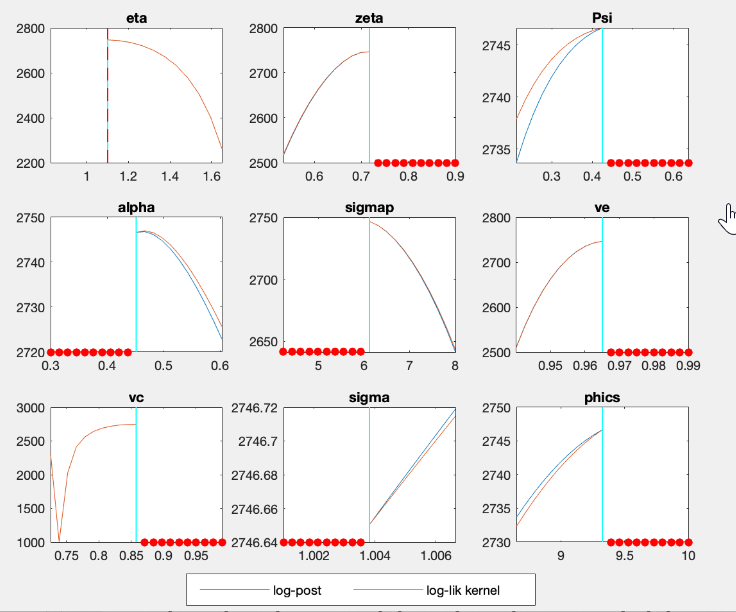
\includegraphics[scale=.55]{Figures/mode_check}
      \end{figure}

    \end{column}%
  \end{columns}


\end{frame}


\begin{frame}{Optimality}
  \begin{itemize}
    \item Kalman filter is basically a least squares estimator\vspace{0.2cm}
    \item If initial conditions and innovations are normal, it is the best predictor! You cannot get better!\vspace{0.2cm}
    \item Otherwise, it is the best linear predictor\vspace{0.2cm}
    \item Can only be used to construct likelihood function for linear (asymptotically) Gaussian state-space systems \vspace{0.2cm}
    \item[$\rightarrow$] works perfectly for first-order approximated DSGE models
    \item[$\rightarrow$] does not work with higher order approximations/non-linearities
  \end{itemize}
\end{frame}




\begin{frame}{Missing observations and mixed frequency}
  \begin{witemize}
    \item Nothing in the Kalman filter recursions requires the involved matrices to be the same in every iteration
    \item Missing observations can thus be easily handled by adjusting the matrices using a selector matrix\\
    $\rightarrow$ Dynare does this automatically
    \item Allows also mixed frequency estimation:
    \begin{itemize}
      \item set up model in the highest frequency
      \item set variables not available at this frequency to missing
      \item define a mapping from the quarterly flow variables in the data to the monthly ones in the model
    \end{itemize}
  \end{witemize}
\end{frame}

\begin{frame}{Making estimation faster}
  \begin{witemize}
    \item Diffuse filter is slower than basic filter: you should weight the benefit of using a non-stationary model
    \item Using a doubling algorithm to compute the unconditional variance is often faster: use estimation option
    \texttt{lyapunov=doubling}
    \item For stationary models: use estimation option
    \texttt{fast\_kalman\_filter}
    \item If you can provide Dynare with an explicit steady state for your
    model with \texttt{steady\_state\_model} block
    \item Use model option \texttt{use\_dll} for medium or large size models
    \item The benefit of the above options is highly model dependent.
    Tests are required to find the best choices for any specific
    model.
  \end{witemize}
\end{frame}

\begin{frame}{Observation equations}
  \begin{witemize}
    \item Up to this point, we have been silent on how to map the observed data to the model variables
    \item This is the topic of specifying the \highlight{observation equations}
    \item The biggest problem is stationarity in the model vs. trends in the data
    \item The guiding principle is: \highlight{the data variable needs to perfectly correspond to a variable defined in the model}
    \item A lengthy treatment of many possible cases is available in \textcite{Pfeifer2013}
    \item We will most of the time consider demeaned growth rates of variables together with a loglinear model
    \item This gives rise to a straightforward observation equation of the form:\\
    \indent \texttt{y\_obs=y-y(-1);}

  \end{witemize}
\end{frame}


\part{References}
%
\begin{frame}[allowframebreaks]{Bibliography}
  \printbibliography
\end{frame}
\end{document}
